%!TEX TS-program = xelatex
%!TEX encoding = UTF-8 Unicode

\documentclass[12pt]{extarticle}
% extarticle is like article but can handle 8pt, 9pt, 10pt, 11pt, 12pt, 14pt, 17pt, and 20pt text

\def \ititle {Origins of Mind}
 
\def \isubtitle {Lecture 08}
 
\def \iauthor {Stephen A. Butterfill}
\def \iemail{s.butterfill@warwick.ac.uk}
\date{}

%for strikethrough
\usepackage[normalem]{ulem}

\input{$HOME/Documents/submissions/preamble_steve_handout}

%logic symbol \leftmodels
\usepackage{MnSymbol}

%\bibpunct{}{}{,}{s}{}{,}  %use superscript TICS style bib
%remove hanging indent for TICS style bib
%TODO doesnt work
\setlength{\bibhang}{0em}
%\setlength{\bibsep}{0.5em}


%itemize bullet should be dash
\renewcommand{\labelitemi}{$-$}

\begin{document}

%\raggedcolumns

\begin{multicols*}{3}

\setlength\footnotesep{1em}


\bibliographystyle{newapa} %apalike

%\maketitle
%\tableofcontents




%--------------- 
%--- start paste

\def \ititle {Logic I}
 
\def \isubtitle {Fast Lecture 02}
 
\begin{center}
 
{\Large
 
\textbf{\ititle}: \isubtitle
 
}
 
 
 
\iemail %
 
\end{center}
 
Readings refer to sections of the course textbook, \emph{Language, Proof and Logic}.
 
 
 
\section{Formal Proof: ∧Elim and ∧Intro}
 
\emph{Reading:} §5.1, §6.1
 
\begin{center}
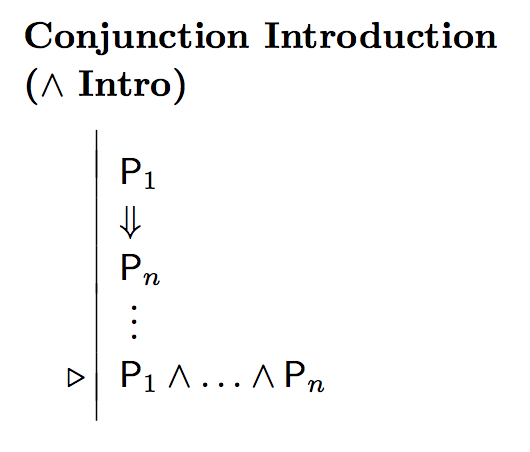
\includegraphics[scale=0.3]{img/rule_conjunction_intro.png}
\end{center}
\begin{center}
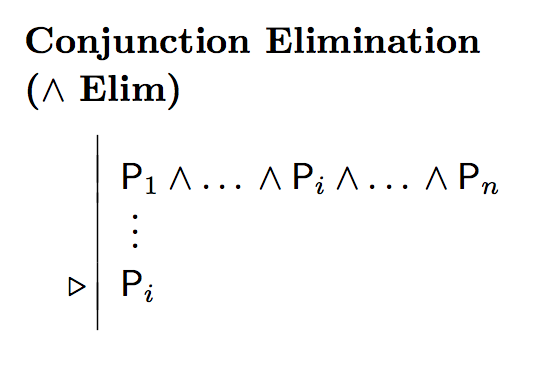
\includegraphics[scale=0.3]{img/rule_conjunction_elim.png}
\end{center}
\begin{center}
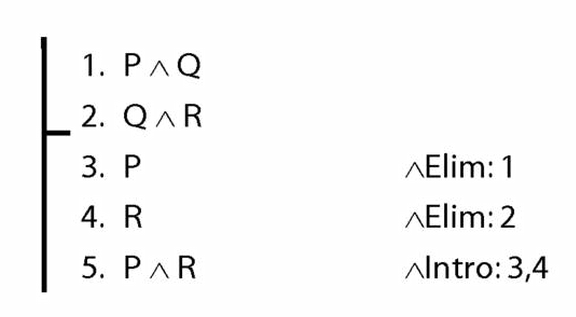
\includegraphics[scale=0.3]{img/proof_unit_21.png}
\end{center}
 
 
\section{∧Intro and ∨Intro: Compare and Contrast}
 
\emph{Reading:} §6.1
 
\begin{center}
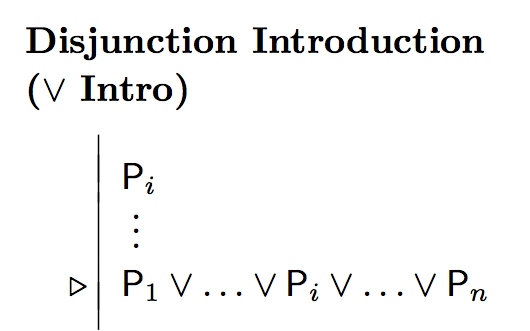
\includegraphics[scale=0.3]{img/rule_disjunction_intro.png}
\end{center}
\begin{center}
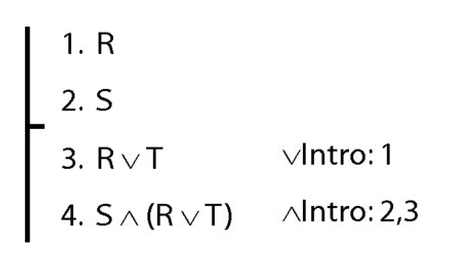
\includegraphics[scale=0.3]{img/proof_unit_212}
\end{center}
\begin{minipage}{\columnwidth}
 
Let us define a new connective with this truth table:
 
\begin{center}
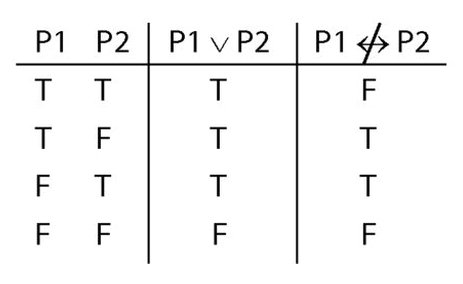
\includegraphics[scale=0.3]{img/tt_not_equivalent.png}
\end{center}
\end{minipage}
 
\begin{minipage}{\columnwidth}
 
The following rule is unacceptable. Why?
 
\begin{center}
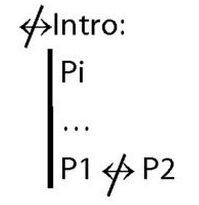
\includegraphics[scale=0.3]{img/rule_not_equivalent_intro_wrong.png}
\end{center}
\end{minipage}
 
 
 
\section{How to Write Proofs}
 
\begin{center}
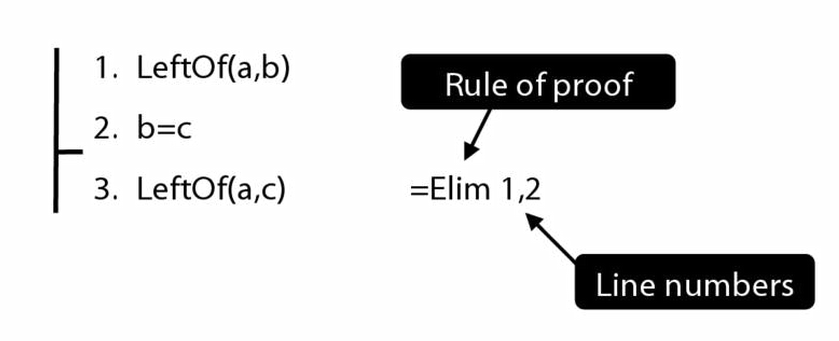
\includegraphics[scale=0.3]{img/how_to_write_proofs.png}
\end{center}
 
\begin{minipage} {\columnwidth}
\section{Rules of Proof for Identity}
 
\emph{Reading:} §2.2
 
\begin{center}
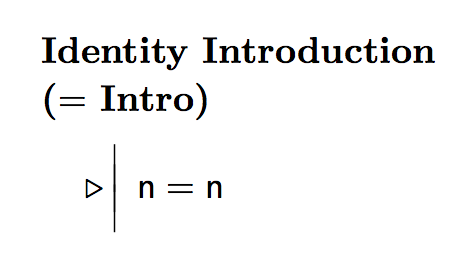
\includegraphics[scale=0.3]{img/rule_identity_intro.png}
\end{center}
\end{minipage}
\begin{center}
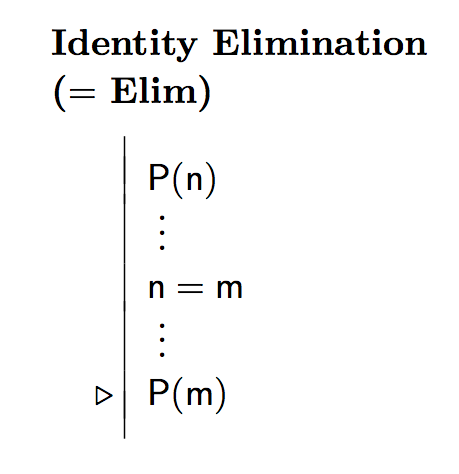
\includegraphics[scale=0.3]{img/rule_identity_elim.png}
\end{center}
\begin{center}
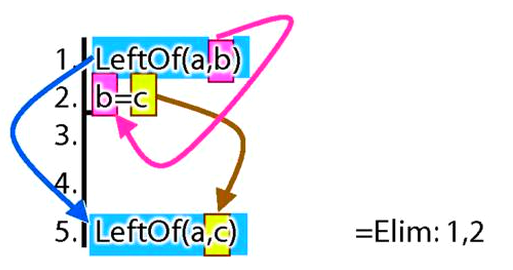
\includegraphics[scale=0.3]{img/proof_identity_example.png}
\end{center}
 
 
\section{DeMorgan: ¬(A ∧ B) $\leftmodels\models$ ¬A ∨ ¬B}
 
\emph{Reading:} §3.6
 
`$\leftmodels\models$' means `is logically equivalent to', so for now `has the same truth table as'.
 
A $\leftmodels\models$ ¬¬A
 
¬(A ∧ B) $\leftmodels\models$ (¬A ∨ ¬B)
 
¬(A ∨ B) $\leftmodels\models$ (¬A ∧ ¬B)
 
A → B $\leftmodels\models$ ¬A ∨ B
 
¬(A → B) $\leftmodels\models$ ¬(¬A ∨ B) $\leftmodels\models$ A ∧ ¬B
 
 
 
\section{→Intro, →Elim}
 
\emph{Reading:} §8.1, §8.2
 
\begin{center}
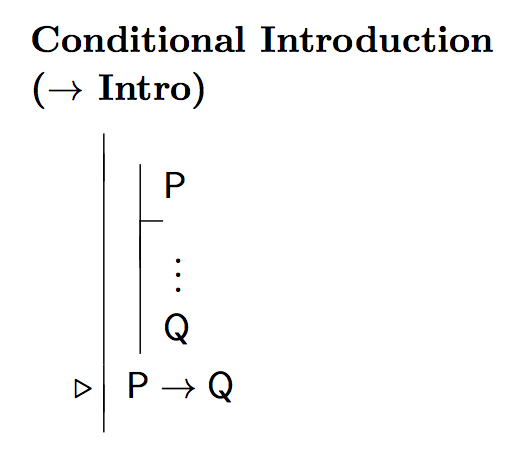
\includegraphics[scale=0.3]{img/rule_arrow_intro.png}
\end{center}
\begin{center}
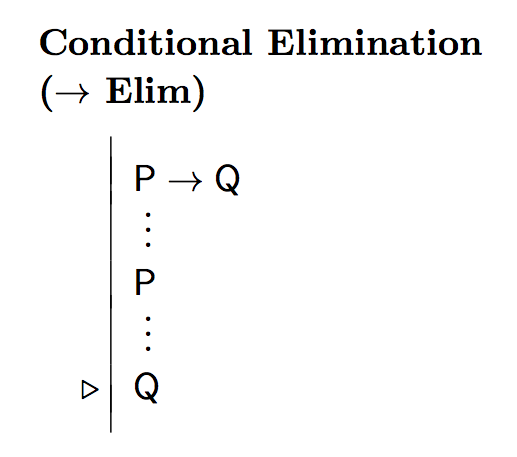
\includegraphics[scale=0.3]{img/rule_arrow_elim.png}
\end{center}
 
 
\section{→Intro: An Example}
 
\begin{center}
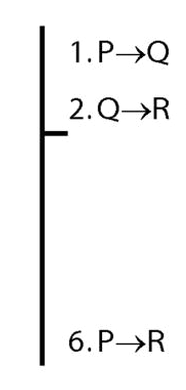
\includegraphics[scale=0.3]{img/proof_arrow_intro.png}
\end{center}
 
 
\section{∨Intro and ∨Elim}
 
\begin{center}
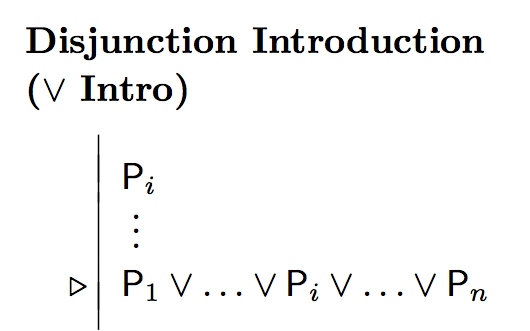
\includegraphics[scale=0.3]{img/rule_disjunction_intro.png}
\end{center}
\begin{center}
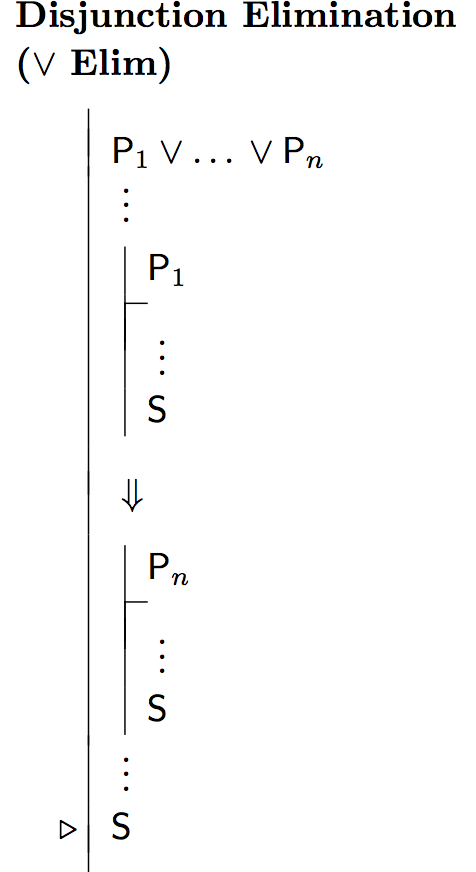
\includegraphics[scale=0.3]{img/rule_disjunction_elim.png}
\end{center}
 
 
\section{∨Elim: An Example}
 
To prove a conclusion from a disjunction, prove it from each disjunct.
 
\begin{center}
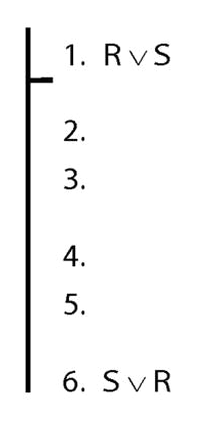
\includegraphics[scale=0.3]{img/proof_disjunction_elim.png}
\end{center}
 
 
\section{¬, $\bot$}
 
\emph{Reading:} §6.3
 
\begin{center}
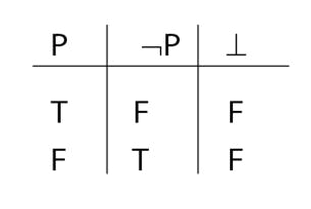
\includegraphics[scale=0.3]{img/tt_contradiction.png}
\end{center}
\begin{center}
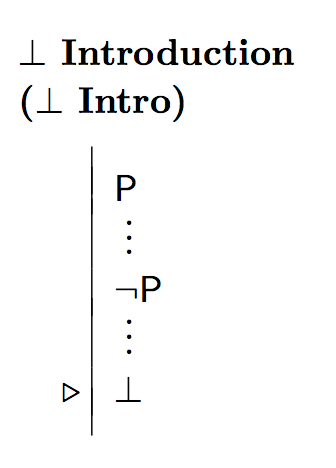
\includegraphics[scale=0.3]{img/rule_contradiction_intro.png}
\end{center}
\begin{center}
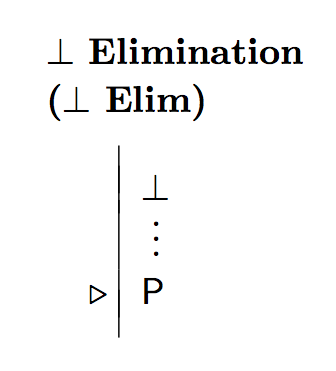
\includegraphics[scale=0.3]{img/rule_contradiction_elim.png}
\end{center}
 
\begin{minipage}{\columnwidth}
\section{¬Elim}
 
\emph{Reading:} §6.3
 
\begin{center}
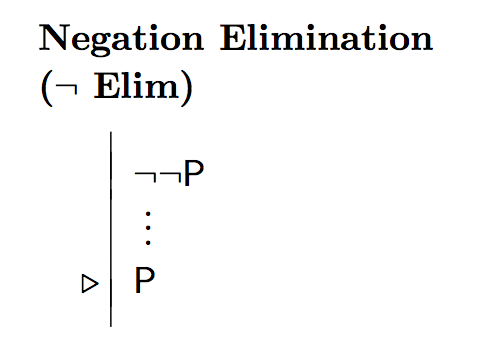
\includegraphics[scale=0.3]{img/rule_negation_elim.png}
\end{center}
\end{minipage} 
 
\section{Scope: A Mistaken Application of ¬Elim}
 
What is wrong with this proof?
 
\begin{center}
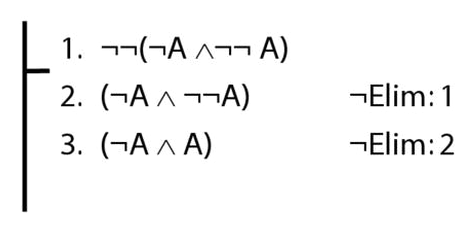
\includegraphics[scale=0.3]{img/proof_negation_elim_wrong.png}
\end{center}
 
\begin{minipage}{\columnwidth}
\section{¬Intro}
 
\emph{Reading:} §5.3, §6.3
 
\begin{center}
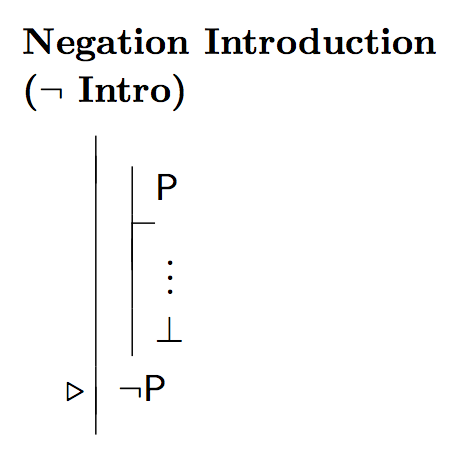
\includegraphics[scale=0.3]{img/rule_negation_intro.png}
\end{center}
 \end{minipage}
 
 
\vfill
\begin{minipage}{\columnwidth}
\section{Exercises}
These exercises will be discussed in seminars the week after this lecture.
The numbers below refer to the numbered exercises in the course textbook, e.g. `1.1' refers to exercise 1.1. on page 39 of the second edition of \emph{Language, Proof and Logic}.
 
\begin{quote}
5.3--5.6
 
3.19
 
4.31
 
6.7--6.12
 
6.18--6.20
 
6.24--6.27
 
*6.40--6.42
 
\end{quote}
\end{minipage}



%--- end paste
%--------------- 
 

\end{multicols*}

\end{document}